\chapter{稳健性与外部验证}
\label{chap:robust}

第五章的主结论有三项。流行初期的误差随规模下降并趋于常数，规模项显著为正。经验交叉点与理论情景区间同量级，但截距与斜率都被放大。阶段转换时，基准偏移掩盖规模效应。主分析有五项设定可能影响这些结论。规模与预测对象来自同一序列，基准用到了整个窗口的数据，且在窗口内固定不变。分析单元是单个州，数据只有一种病和一个报告系统。本章逐项改变这些选择。第~\ref{sec:rob-forest}~节先汇总各规格下的经验交叉点。第~\ref{sec:rob-iv}~节至第~\ref{sec:rob-tv}~节依次改变规模测度、基准的信息集和基准的时变性。第~\ref{sec:rob-pool}~节用全国汇总序列考察空间汇总。第~\ref{sec:rob-external}~节引入两组外部数据。第~\ref{sec:rob-discussion}~节讨论结果对监测工作的含义及其与已有研究的关系。

\section{各规格的汇总}
\label{sec:rob-forest}

图~\ref{fig:forest} 汇总了第五章与本章各规格下的经验交叉点 $b/a$。所有规格的规模项都为正，凡给出区间的规格，区间都不含零。交叉点则在 10.6--124.7 之间变化，跨越一个数量级。NHSN 数据的各规格大多落在 10--75 之间，外部数据的交叉点更大。变化的方向有规律可循。分母噪声越大、基准对小规模越敏感，斜率越大，交叉点越靠右；剔除极端值则把交叉点推向左侧。规模项为正这一定性结论在所有规格下保持，交叉点的具体数值则取决于规格，只能作为量级参考。

\begin{figure}[!tbp]
  \centering
  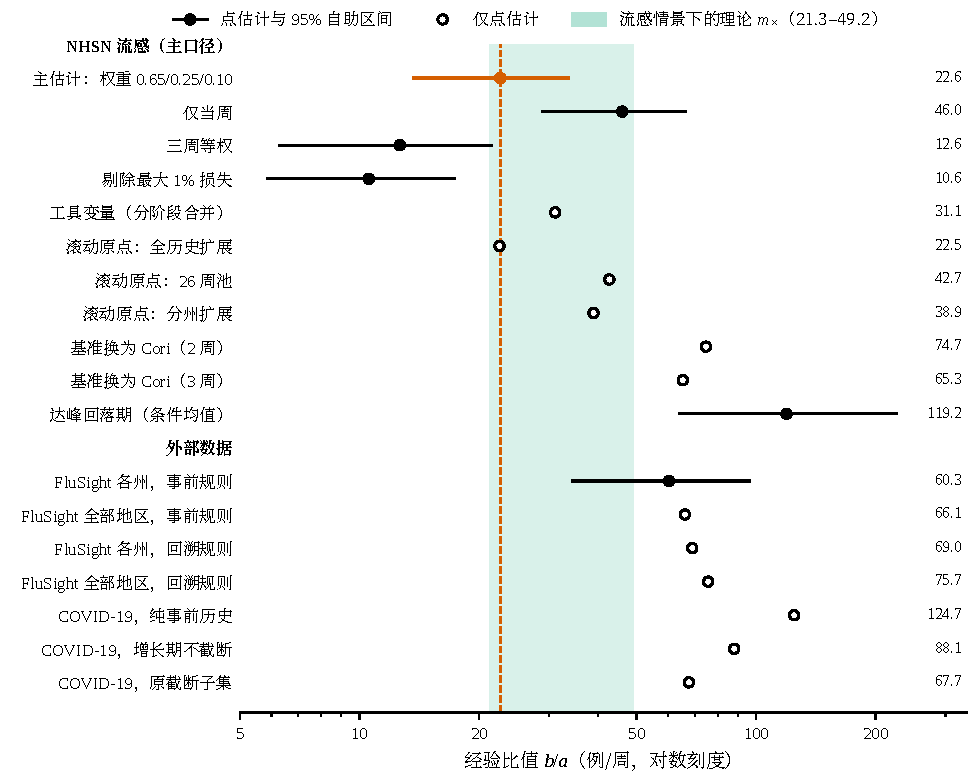
\includegraphics[width=\textwidth]{figures/fig_6_1_mx_forest.pdf}
  \caption{各规格下的经验交叉点 $b/a$。横线为 95\% 区间（只有部分规格提供），阴影为理论情景区间 21.3--49.2，竖直虚线为主估计 22.6，右侧列出点估计。上部为 NHSN 数据的不同规格，下部为外部数据。}
  \label{fig:forest}
\end{figure}

\section{替代性规模测度与工具变量}
\label{sec:rob-iv}

主分析中的 $D_t$ 与 $C_{t+1}$ 来自同一序列，同期测度可能带来两类问题。$D_t$ 含报告噪声，作为回归元时会造成衰减偏误\citep{fuller1987measurement, carroll2006measurement}；规模还可能与当期传播水平相关，规模大的州周恰好处在传播较快的时期。两种情形下 $1/D_t$ 都与回归误差相关，普通最小二乘与可行广义最小二乘都不一致。

工具变量法要求工具与 $1/D_t$ 相关，而与误差项无关。这里取滞后 3--5 周的规模作为 $1/D_t$ 的工具，在流行季内合并样本上做两阶段最小二乘\citep{wooldridge2010econometric}。各州的规模在季内平稳变化，三到五周前的规模与当前规模高度相关；滞后足够长时，旧规模中的报告噪声与当前分母中的噪声相互独立。合并样本要求每个州周都有完整的滞后，共 1,051 个州周，与主样本不同，比较应在同一样本上进行。区间由 10,000 次按州聚类的重抽给出。

表~\ref{tab:iv} 列出合并样本与分季的结果。合并样本的 $b_{\mathrm{iv}}=2.53$（95\% 区间 1.11--4.11），同一样本上的普通最小二乘为 1.35。两者之差的区间为 0.30--2.11，不含零，对应的交叉点为 31.1。改用子样本自身的均值作基准，$b_{\mathrm{iv}}=2.85$（1.32--4.55），交叉点 35.3。第一阶段 $F$ 统计量为 1,147.1，按州聚类后为 312.9，远高于弱工具的常用门槛 10。分季来看，三个流行季的 $b_{\mathrm{iv}}$ 都为正，区间都不含零，点估计都高于同季的普通最小二乘。差值只在 2024--25 季的区间不含零。另两季的区间含零，单季样本只有 273--420 个州周，精度有限。

\begin{table}[!tbp]
  \centering
  \caption{以滞后规模为工具的两阶段最小二乘估计}
  \label{tab:iv}
  \small
  \begin{tabular}{@{}lcccccc@{}}
    \toprule
    样本 & 州周数 & $b_{\mathrm{iv}}$（95\% 区间） & $b_{\mathrm{ols}}$ & 差值的 95\% 区间 & $b_{\mathrm{iv}}/a_{\mathrm{iv}}$ & 聚类 $F$ \\
    \midrule
    2022--23 季 & 273 & 3.28（0.90--6.47） & 1.89 & $-0.15$--3.89 & 60.2 & 94.5 \\
    2023--24 季 & 358 & 2.19（0.65--4.31） & 1.68 & $-0.55$--1.74 & 58.5 & 119.4 \\
    2024--25 季 & 420 & 3.61（0.73--7.23） & 1.83 & 0.01--3.47 & 30.5 & 76.8 \\
    合并（季内均值） & 1,051 & 2.53（1.11--4.11） & 1.35 & 0.30--2.11 & 31.1 & 312.9 \\
    合并（子样本均值） & 1,051 & 2.85（1.32--4.55） & 1.46 & 0.43--2.41 & 35.3 & 312.9 \\
    \bottomrule
  \end{tabular}

  \vspace{4pt}
  {\small 注：工具为滞后 3--5 周的规模；区间由 10,000 次按州聚类的重抽得到；聚类 $F$ 为按州聚类的第一阶段 $F$ 统计量。}
\end{table}

$b_{\mathrm{iv}}$ 高于普通最小二乘，与回归元含噪造成的衰减偏误方向一致。工具变量斜率高于普通最小二乘，与第五章第~\ref{sec:emp-inflation}~节并不矛盾。分母噪声通过两条途径影响斜率：进入 $G_t$ 时抬高小规模处的损失，使斜率变大；进入回归元 $1/D_t$ 时稀释斜率，使斜率变小。式~\eqref{eq:b-delta} 描述前一条途径，工具变量处理的是后一条途径。排除限制要求滞后规模只通过当前规模影响损失，这一条件无法检验；若滞后规模与当前的传播阶段相关，工具变量估计仍有偏。因此工具变量结果只说明，在替代性规模测度下规模项保持为正。

\section{事前基准}
\label{sec:rob-exante}

主分析的基准 $\Rbar_{\mathrm{early}}$ 用整个窗口的数据计算，属于回顾性口径。实时监测中，当周只能使用过去的信息。若规模效应只是回顾性基准的产物，换用事前基准后应当消失。这里考察三种只含过去信息的基准。全部州的历史扩张窗取当周之前所有州周增长比的均值。26 周滚动池取当周之前 26 周内所有州周的均值。逐州扩张窗取同一州此前各周的均值。

表~\ref{tab:exante} 的上半部分给出结果。三种事前基准下误差整体上升，截距 $a$ 在 0.222--0.406 之间，是主估计的 2.2--4.1 倍；斜率 $b$ 在 9.16--13.27 之间，所有重抽的 $b$ 都为正。交叉点为 22.5--42.7，仍与理论情景区间同量级。截距在平均损失中的份额随口径在 39\%--55\% 之间移动。

\begin{table}[!tbp]
  \centering
  \caption{事前基准与时变基准下的误差}
  \label{tab:exante}
  \small
  \begin{tabular}{@{}lccccc@{}}
    \toprule
    基准 & 州周数 & 平均损失 & 截距 $a$ & 斜率 $b$（95\% 区间） & $b/a$ \\
    \midrule
    \multicolumn{6}{@{}l}{事前基准} \\
    全部州历史扩张窗 & 1,267 & -- & 0.406 & 9.16（5.82--12.88） & 22.5 \\
    26 周滚动池 & 1,267 & -- & 0.222 & 9.46（6.76--12.81） & 42.7 \\
    逐州扩张窗 & 1,260 & -- & 0.341 & 13.27（9.14--18.29） & 38.9 \\
    \midrule
    \multicolumn{6}{@{}l}{时变基准} \\
    阶段均值（主估计） & 1,267 & 0.181 & 0.0991 & 2.24（1.50--3.02） & 22.6 \\
    Cori 滑动窗（1 周） & 1,197 & 0.436 & -- & -- & -- \\
    Cori 滑动窗（2 周） & 1,244 & 0.288 & 0.0812 & 6.06 & 74.7 \\
    Cori 滑动窗（3 周） & 1,251 & 0.249 & 0.0763 & 4.98 & 65.3 \\
    朴素预测（下周等于本周） & 1,267 & 0.637 & -- & -- & -- \\
    \bottomrule
  \end{tabular}

  \vspace{4pt}
  {\small 注：每种基准的损失都以该基准自身的预测值归一化；“--”表示未作相应计算。}
\end{table}

截距的上升有明确来源。事前基准只能用过去的增长比外推，流行初期增长比本身在逐周变化，过去的均值与当周的阶段水平之间存在系统差距。按第四章式~\eqref{eq:mse-decomp}，这一差距进入条件偏差项，与规模无关，因而表现为截距上升。斜率同样上升，但规模项为正的结论不变。事前基准解决了基准的前视问题，没有解决窗口划定本身用到事后信息的问题，后者在第~\ref{sec:concl-limits}~节讨论。

\section{时变基准}
\label{sec:rob-tv}

阶段均值基准在整个窗口内固定不变。若改用逐周更新的基准，规模效应是否仍然存在，截距能否降低，是第五章达峰期结果留下的问题。这里用 \citet{cori2013new} 的滑动窗口方法估计 $R_t$，以最近 1、2、3 周的报告数之和除以对应的感染压力之和，作为下一周增长比的预测。作为对照，朴素预测直接以本周病例数预测下周。

表~\ref{tab:exante} 的下半部分给出平均损失。阶段均值基准为 0.181，Cori 滑动窗随窗宽由 1 周增至 3 周，从 0.436 降到 0.249，朴素预测为 0.637。对 Cori 基准的损失拟合式~\eqref{eq:affine}，2 周窗 $a=0.0812$，$b=6.064$，交叉点 74.7；3 周窗 $a=0.0763$，$b=4.984$，交叉点 65.3。两种窗宽的截距都低于阶段均值基准的 0.0991，斜率则是后者的 2--3 倍。

图~\ref{fig:baselines} 按规模分箱比较四种基准。按各自预测值归一化时（图~\ref{fig:baselines}a），$D_t<100$ 的三箱中阶段均值基准的损失最低，Cori 2 周窗在最小箱为 0.658，是阶段均值基准 0.329 的两倍。$D_t\geq100$ 的三箱中两种 Cori 基准都略低于阶段均值基准，例如 $[100,250)$ 箱的 0.090 和 0.087 对 0.112。朴素预测在所有箱中损失最高。统一以 $\Rbar_{\mathrm{early}}$ 归一化、只用 Cori 2 周窗可用的 1,244 个州周时（图~\ref{fig:baselines}b），Cori 2 周窗的平均损失为 0.223，朴素预测为 0.274；在最大箱中朴素预测降到 0.064，低于阶段均值基准的 0.105。

\begin{figure}[!tbp]
  \centering
  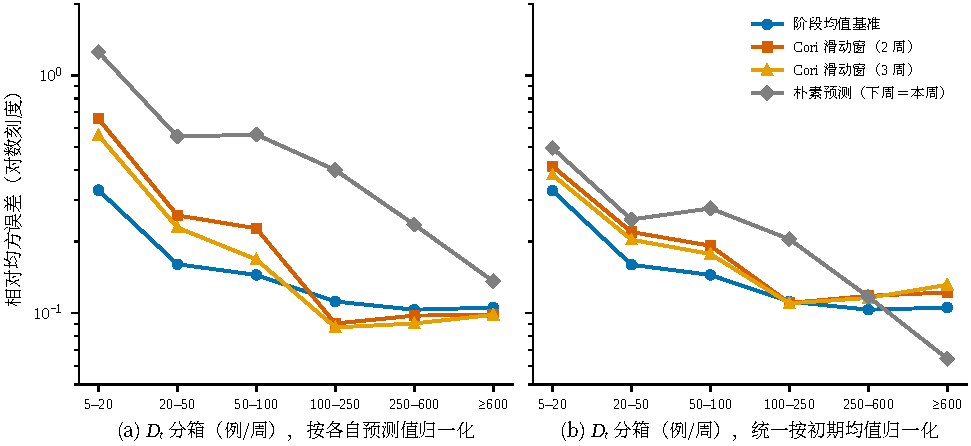
\includegraphics[width=\textwidth]{figures/fig_6_2_baselines.pdf}
  \caption{流行初期四种预测基准在各规模分箱上的相对均方误差，纵轴为对数刻度。（a）每种基准的损失以其自身预测值归一化，各基准使用各自可计算的样本；（b）四种基准的损失统一以初期均值 $\overline{R}_{\mathrm{early}}$ 归一化，样本限于 Cori 2 周窗可计算的 1,244 个州周。}
  \label{fig:baselines}
\end{figure}

分箱结果说明了截距的构成。时变基准用近期数据估计 $R_t$，自身就是一个带抽样噪声的比值，规模小时噪声大，斜率因此更陡。规模大时抽样噪声可以忽略，时变基准能跟踪各州各周增长水平的变化，误差低于固定基准。大规模处的误差下降意味着，阶段均值基准的截距中有一部分来自可由近期数据预测的增长水平变化。这部分误差不属于规模无法消除的环境方差。这与第五章截距随回溯滞后上升的结果一致，$R_t$ 的时间相关使近期数据含有当期传播水平的信息。时变基准降低截距的幅度有限，最大箱中 Cori 2 周窗仍有 0.098，截距不会因换用时变基准而消失。

\section{空间汇总}
\label{sec:rob-pool}

第三章式~\eqref{eq:pooling} 表明，汇总 $J$ 个辖区后环境底板降为 $v_R\bar c+v_R(1-\bar c)/J$，降幅取决于辖区间环境波动的平均相关 $\bar c$。全国加总序列提供了一个检验。三个流行初期窗口中，全国序列共 28 周，平均规模约 6,662 例/周，平均增长比 1.539，平均损失 0.0348，中位数 0.0115。按主估计 $b=2.243$，规模项 $b/D$ 约为 0.0003，可以忽略，全国序列的损失几乎全部是环境底板。

以州级截距 0.0991 作为单辖区的底板，比值 $0.0348/0.0991=0.351$。代入式~\eqref{eq:pooling}，$J=51$ 时
\begin{equation}
  \bar c+\frac{1-\bar c}{51}=0.351 ,
  \label{eq:cbar}
\end{equation}
解得 $\bar c\approx0.34$。各州的环境波动只有约三分之一是全国共同的，其余部分在汇总中相互抵消。若各州完全同步（$\bar c=1$），汇总不会降低底板；若完全独立（$\bar c=0$），底板会降到州级的 1/51。实际降幅介于两者之间。

这一推算较为粗略。全国序列只有 28 周，平均损失的抽样误差较大。州级截距 0.0991 本身被分母噪声和 $G_t$ 的口径放大，第五章已说明它高于真实的 $v_R/\Rbar^2$。全国序列的平均增长比 1.539 也不同于州级的 1.6706，两者归一化的尺度不同。$\bar c\approx0.34$ 只能当作量级。在方向上，汇总确实把环境底板降到州级的三分之一左右，与命题~\ref{prop:allocation} 的时间方向结论相互补充。时间上增加期数与空间上增加辖区，都能降低平均传播水平估计的误差。两者的效果分别受时间相关与空间相关的限制。

\section{外部数据}
\label{sec:rob-external}

\subsection{FluSight 集成预测}

前述分析都使用以阶段均值为核心的简单基准。实际的流感预测由多个团队的模型集成给出。FluSight 是美国疾病控制与预防中心组织的流感住院前瞻预测，这里使用其 2022--23 季的集成预测\citep{mathis2024evaluation}，相关评价框架见文献\citep{reich2019accuracy, cramer2022evaluation}。集成预测给出下一周住院数的预测值 $\widehat Y$。主口径以 $\widehat Y$ 作为规模测度并据此筛选样本，筛选只用事前信息。

以 $\widehat Y\geq5$ 筛选州级样本（$N=1{,}177$），对相对误差平方拟合式~\eqref{eq:affine}，得到 $a=0.1295$（95\% 区间 0.1020--0.1633），$b=7.805$（5.358--10.526），交叉点 60.3（34.5--95.9）。表~\ref{tab:external} 列出另外三种筛选口径，交叉点为 66.1、69.0 和 75.7。集成预测的截距与阶段均值基准接近，斜率是后者的三倍以上，交叉点相应更大。

把集成预测在各流行阶段内的相对均方误差拆成均值偏差平方与阶段内方差两部分，均值偏差平方在上升期（$N=216$）占 32.3\%，在峰期（$N=206$）占 15.5\%，在回落期（$N=755$）占 1.5\%。第五章中阶段均值基准在达峰期的偏差占比为 88.9\%。集成预测在峰期能较好地跟踪阶段变化，偏差占比低得多，上升期的偏差占比最高，与预测模型对增长起点反应滞后的情形相符，现有分解不足以确定其原因。两组数字来自不同的模型、季节和样本，只能作方向性参照。

\subsection{欧洲 COVID-19 早期序列}

第二组外部数据是欧洲 11 国 2020 年 2--4 月的 2019 冠状病毒病序列\citep{flaxman2020estimating}，单元为国家。三种口径的结果列于表~\ref{tab:external}。只用过去信息构造基准时，$N=404$，$b=33.92$（14.60--74.99），交叉点 124.7；只取增长期为 88.1，截断子样本为 67.7。三种口径的规模项都为正，交叉点都高于 NHSN 主估计。

\begin{table}[!tbp]
  \centering
  \caption{外部数据的仿射误差模型估计}
  \label{tab:external}
  \small
  \begin{tabular}{@{}llcccc@{}}
    \toprule
    数据 & 口径 & 单元数 & 截距 $a$ & 斜率 $b$（95\% 区间） & $b/a$ \\
    \midrule
    FluSight 2022--23 & 州，事前 $\widehat Y\geq5$ & 1,177 & 0.129 & 7.80（5.36--10.53） & 60.3 \\
     & 全部地区，事前 & 1,203 & 0.122 & 8.07 & 66.1 \\
     & 州，事后 $C\geq5$ & 1,137 & 0.124 & 8.52 & 69.0 \\
     & 全部地区，事后 $C\geq5$ & 1,163 & 0.116 & 8.81 & 75.7 \\
    \midrule
    欧洲 COVID-19 & 纯事前基准 & 404 & 0.272 & 33.92（14.60--74.99） & 124.7 \\
     & 仅增长期 & 318 & 0.210 & 18.53（7.13--44.10） & 88.1 \\
     & 截断子样本 & 307 & 0.189 & 12.76（7.25--20.01） & 67.7 \\
    \bottomrule
  \end{tabular}

  \vspace{4pt}
  {\small 注：FluSight 的单元为州周，聚类单元为州；欧洲 COVID-19 的观测按国家与时间索引，聚类单元为国家。}
\end{table}

COVID-19 序列的交叉点更大，与该序列更高的平均增长比相符。三种口径的平均增长比在 2.9--3.5 之间，按式~\eqref{eq:var-average}，规模项 $A$ 随 $\Rbar$ 增大。2020 年初各国检测能力变化较快，报告率不稳定也可能抬高斜率。两组外部数据的病种、预测方法和报告系统都与 NHSN 不同，交叉点不宜直接比较大小。外部数据支持的结论是定性的：误差中存在随规模下降的成分，且在规模达到数十至一百余例后趋于平缓。

\section{讨论}
\label{sec:rob-discussion}

\subsection{对监测工作的含义}

全文的核心区分是估计目标。同一份病例数据，用来判断本周是否在增长，与用来估计一段时期的平均传播水平，对规模的需求相差很大。前者属于目标Ⅰ，方差随规模趋于零，第四章第~\ref{sec:design-test}~节的计算表明，要稳定检出 15\% 的增长，所需规模约为交叉点的十倍。后者属于目标Ⅱ，规模超过 $\mx$ 以后误差主要来自环境波动，扩大病例捕获的回报迅速变小。

由此可以提出双轨监测的思路。预警类问题对应目标Ⅰ，规模越大越好，资源应投向报告及时、覆盖完整的单元。趋势类问题对应目标Ⅱ，规模达到交叉点的量级后，更有效的做法是增加观测期数，或汇总多个辖区。命题~\ref{prop:allocation} 与式~\eqref{eq:pooling} 分别给出时间与空间两个方向的收益，第~\ref{sec:rob-pool}~节的全国序列把环境底板降到州级的三分之一左右。

阶段转换时的误差需要另一类对策。达峰期以初期均值为基准时，88.9\% 的损失来自基准偏移，规模再大也无济于事；换用阶段自身基准后，规模项重新为正。时变基准在大规模处降低了误差，FluSight 集成预测在峰期的偏差占比只有 15.5\%，两者都表明能跟踪阶段变化的模型可以压低偏差项。在流行阶段转换时，应优先更新基准模型，同时维持足以控制规模项的病例数。

数据质量的监控也可以从第五章得到启示。自愿填报期 $G_t$ 的标准差大幅扩张，四分位距与中位绝对偏差几乎不变，扰动集中在少数极端周。这类结构性扰动比均匀漏报更难处理。用稳健离散度监控整体噪声，用标准差与偏度识别结构性扰动，两类指标并用，可以较早地发现填报行为的变化。

\subsection{与已有研究的关系}

Parag 等的信息论结果针对当期再生数，Fisher 信息随病例数线性增长\citep{parag2022quantifying, parag2022fundamental}，这与目标Ⅰ的结论一致。本文补充的是目标Ⅱ：环境方差 $v_R$ 给出一个规模无法突破的底板，交叉点 $\mx$ 把这一底板换算成具体的病例数。生态学区分环境随机性与人口随机性\citep{engen1998demographic, rohani2002determinism}，前者影响整个种群，后者随种群规模增大而平均掉；第三章的方差分解在监测设计中给出了这一区分的对应。

预测评价文献通常按地区或时期报告误差\citep{reich2019accuracy, cramer2022evaluation}。本章的 FluSight 结果表明，集成预测的误差同样含有随规模下降的成分与不随规模下降的底板。按相对误差比较不同规模的地区时，小规模地区的误差偏高有一部分来自规模项，这部分与模型优劣无关。把规模作为协变量纳入预测评价，可以把模型差异与规模差异分开。

\section{本章小结}
\label{sec:rob-summary}

本章在替代规格、空间汇总与外部数据下检验了第五章的结论。以滞后规模为工具的两阶段最小二乘给出 $b_{\mathrm{iv}}=2.53$，高于同一样本的普通最小二乘，方向与衰减偏误一致。三种事前基准下截距上升到主估计的 2--4 倍，规模项仍然为正。Cori 滑动窗口基准在小规模处误差更大，在大规模处略低于阶段均值基准，说明截距中有一部分是可由近期数据预测的增长水平变化。全国汇总序列的损失约为州级截距的三分之一，粗略推算的州间环境相关约为 0.34。FluSight 集成预测与欧洲 COVID-19 序列中规模项都为正，交叉点为 60.3--124.7。

所有规格下规模项都为正，经验交叉点则在 10.6--124.7 之间变化。规模的收益随规模递减、存在环境底板这一定性结论是稳健的；交叉点的具体数值依赖规格、病种与预测方法，只能作为量级参考。这些结果对监测设计的含义已在第~\ref{sec:rob-discussion}~节讨论，第七章将其归纳为实践建议。
